\documentclass[10pt,twocolumn]{article}

\usepackage[letterpaper,margin=0.78in,columnsep=0.28in]{geometry}
\usepackage[T1]{fontenc}
\usepackage[utf8]{inputenc}
\usepackage{mathptmx}
\usepackage{microtype}
\usepackage{amsmath,amssymb,amsthm}
\usepackage{graphicx}
\graphicspath{{../results/figures/}}
\usepackage{booktabs}
\usepackage{multirow}
\usepackage{tikz}
\usetikzlibrary{arrows.meta,positioning,fit,backgrounds,calc,shapes.geometric}
\usepackage{algorithm}
\usepackage[noend]{algpseudocode}
\usepackage{enumitem}
\usepackage{xcolor}
\usepackage{caption}
\usepackage[colorlinks=true,allcolors=Navy]{hyperref}
\usepackage{url}
\Urlmuskip=0mu plus 1mu\relax
\def\UrlBreaks{\do\/\do\-\do\.}
\usepackage{cleveref}

\definecolor{Navy}{HTML}{1B3A5C}
\definecolor{Brick}{HTML}{B03A2E}
\definecolor{Olive}{HTML}{6B7D2F}
\definecolor{Plum}{HTML}{7D3C98}
\definecolor{Pale}{HTML}{F4F1EA}

\captionsetup{font=small,labelfont=bf,skip=5pt}
\setlist{nosep,leftmargin=1.2em}

\newtheorem{theorem}{Theorem}
\newtheorem{proposition}{Proposition}
\newtheorem{definition}{Definition}
\theoremstyle{remark}
\newtheorem{remark}{Remark}

\newcommand{\Gen}{\textsf{Gen}}
\newcommand{\Rep}{\textsf{Rep}}
\newcommand{\KDF}{\textsf{KDF}}
\newcommand{\Sign}{\textsf{Sign}}
\newcommand{\Vf}{\textsf{Vf}}
\newcommand{\Ext}{\textsf{Ext}}
\newcommand{\emb}{f_\theta}
\newcommand{\bits}{\{0,1\}}
\newcommand{\hinf}{\mathbf{H}_\infty}
\newcommand{\hinft}{\widetilde{\mathbf{H}}_\infty}

\title{\vspace{-2.2em}\bfseries ADAMAS: Cryptographically Binding a Diamond's\\
Physical Signature to Its On-Chain Provenance}

\author{%
\normalsize Aarush Kandukoori\\[1pt]
\small School of Computer Science, Carnegie Mellon University\\
\small \texttt{akandukoori@andrew.cmu.edu}
}
\date{}

\begin{document}
\maketitle

\begin{abstract}
\noindent
Distributed ledgers give diamond provenance systems tamper-evident records. They
do not give those records any verifiable connection to the physical stones the
records describe. Every deployed platform closes that gap with a trusted
operator: a laboratory scans a stone, an algorithm declares a match against a
stored template, and the ledger faithfully records the operator's assertion. An
adversary who substitutes stones between checkpoints, compromises a scanner, or
replays a stored measurement defeats the system while leaving the chain
internally consistent. We call this the \emph{binding gap}.

We present ADAMAS, a protocol that derives a cryptographic key directly from a
stone's crystallographic defect structure and makes possession of the physical
stone a prerequisite for every provenance operation. ADAMAS has three layers: a
learned $SE(3)$- and permutation-invariant embedding of the internal inclusion
constellation that provides alignment-free screening; a registration-and-vault
stage that converts the inclusion point set into a reproducible key; and a
challenged-interrogation layer over photoluminescence and nitrogen-vacancy
sub-volumes that defeats replay and constrains a compromised sensor. Custody
transfers are co-signed by the stone itself, so a record cannot move without the
object.

We derive a feasibility bound relating bit error rate, per-bit min-entropy, and
extractable key length, and evaluate the pipeline on a synthetic population of
1{,}000 simulated stones. Three findings shape the design. First, learned
within-class whitening reduces the screening equal error rate from
$8.9\times10^{-2}$ to $1.9\times10^{-2}$, but the resulting alignment-free
descriptor carries only $\approx 55$ bits of extractable entropy, far below what
a $128$-bit binding requires; a single-stage fuzzy extractor over global
invariants is structurally insufficient. Second, geometry alone cannot separate
natural from laboratory-grown stones ($200/200$ synthetic CVD substitutes pass
the geometric screen), whereas the spectroscopic block separates them at
$99.8\%$ accuracy: the material-class gate must be spectroscopic. Third, the
registered point-set vault reaches $90$-bit security at a $97\%$ unlock rate
with $14$ mapped inclusions, and $128$-bit security requires reliably mapping
$\geq 20$ inclusions per stone, which is an instrument specification rather than
a protocol parameter. We also find that an adversary holding $90\%$ of a stone's
inclusion map unlocks the vault with probability $0.49$, which makes the routine
publication of clarity plots a live disclosure risk.

We argue that unforgeability in the absolute sense is unattainable, and that the
achievable goal is a reduction: forgery becomes equivalent to atomic-scale
replication of a defect constellation, compromise of an attested instrument, or
possession of the genuine stone, with each made detectable and attributable. All
evaluation is simulation on synthetic data; we specify the physical study with
graded stones that would validate or refute it.
\end{abstract}

\vspace{0.6em}

\section{Introduction}

In 2024 a gemological laboratory received a six-carat stone bearing the girdle
inscription of a certified natural diamond. The inscription was authentic in the
sense that it matched a real report. The stone was not: photoluminescence (PL)
spectroscopy revealed a silicon-vacancy doublet near $737$~nm, diagnostic of
chemical vapor deposition growth. The substitution was caught because a
laboratory happened to run spectroscopy, and because the observed inclusions
disagreed with the plot on the referenced report. Absent that scrutiny, a
digitally impeccable provenance record would have accompanied the wrong
object~\cite{igi2024}.

That incident is the whole problem in miniature. A provenance record is a claim
about a physical object. Cryptography and consensus can make the claim
tamper-evident, ordered, and attributable. Neither can make the claim
\emph{true}. The step where a measurement of matter becomes a statement in a
ledger is the step where an adversary operates, and it is the step that
distributed-ledger provenance systems have historically delegated to a trusted
operator.

\paragraph{Why now.} The economic pressure on this seam is increasing sharply.
Laboratory-grown stones are visually and gemologically close to natural ones,
sell for a fraction of the price, and have taken a large share of the
engagement market, while natural rough prices have fallen for several
consecutive years~\cite{tnw2026}. The premium attached to a natural-origin
certificate is therefore both larger in relative terms and easier to
counterfeit, since the counterfeit substrate is cheap and abundant. In parallel,
the industry has consolidated around ledger-based provenance: De Beers launched
Tracr in 2018, opened it to the wider industry in 2023, and in May 2026 the
Gemological Institute of America (GIA) agreed to acquire a $30\%$ shareholding
as the platform moves toward independence~\cite{gia2026,debeers2026}. More than
five million rough diamonds have been registered at source, and since January
2025 all newly sourced De Beers rough of one carat and above is
registered~\cite{gia2026}. The infrastructure that a binding attack would target
is now real, large, and load-bearing.

\paragraph{The binding gap.} Deployed systems bind records to stones by
\emph{algorithmic matching under a trusted operator}. Sarine's Diamond Journey,
for example, scans a rough stone, plans the cut, re-scans the polished result,
and confirms identity by matching proportions, inclusions, and other features
against the recorded plan; the registration then transfers to the new
owner~\cite{sarine_journey,sarine_tech}. This is a genuine technical
achievement, and it is exactly what the industry needs for logistics. As a
security mechanism it has four structural properties an adversary can use:

\begin{enumerate}
\item \textbf{The comparison is a similarity threshold, not a key.} A match
produces a boolean from a trusted process. Nothing cryptographic is derived from
the stone, so nothing the stone produces can be independently verified by a
third party.
\item \textbf{The template must be stored in the clear} to be compared against,
so whoever holds the registry holds every fingerprint, and a registry breach is
a permanent, unrevocable compromise.
\item \textbf{There is no freshness.} A stored scan replayed by a compromised or
merely lazy scanner is indistinguishable from a live measurement.
\item \textbf{The stone never signs anything.} Custody transfers are authorized
by parties, so a record can move while the object stays still, or vice versa.
\end{enumerate}

\paragraph{What is actually achievable.} We state our position plainly, because
the framing of the problem invites overclaiming. A protocol cannot make physical
provenance unforgeable. Any system that turns matter into bits contains a sensor,
and a sufficiently compromised sensor can assert anything. What a protocol
\emph{can} do is reduce forgery to a small set of irreducible capabilities and
make each one expensive, detectable, and attributable. ADAMAS targets the
reduction in \Cref{fig:reduction}: to forge provenance an adversary must either
replicate a defect constellation at atomic scale, compromise an attested
instrument and defeat its challenge-response, or physically hold the genuine
stone. The third case is uninteresting, since an adversary holding the genuine
stone would rather sell it.

\begin{figure}[t]
\centering
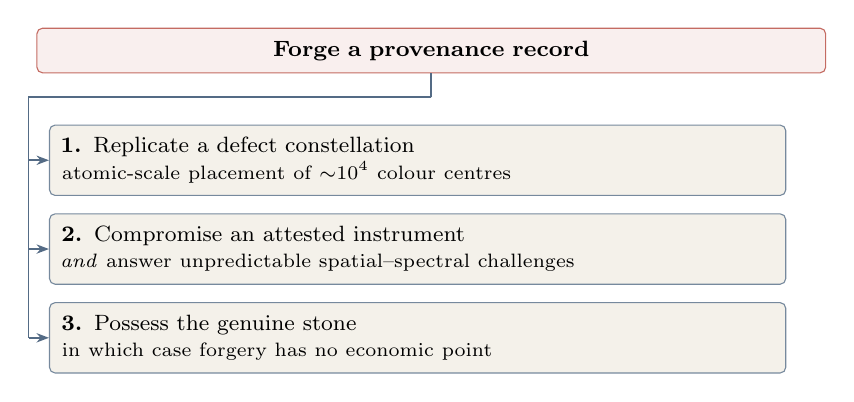
\begin{tikzpicture}[
  font=\footnotesize,
  goal/.style={draw=Brick!75,fill=Brick!8,rounded corners=2pt,inner sep=4.5pt,
               align=center,text width=0.80\columnwidth},
  path/.style={draw=Navy!60,fill=Pale,rounded corners=2pt,inner sep=4.5pt,
               align=left,text width=0.745\columnwidth},
  ar/.style={-{Stealth[length=4.5pt]},Navy!75,semithick}]
\node[goal] (a) {\textbf{Forge a provenance record}};
\node[path,below=6.5mm of a.south west,anchor=north west,xshift=1.6mm] (b)
  {\textbf{1.} Replicate a defect constellation\\
   \scriptsize atomic-scale placement of ${\sim}10^{4}$ colour centres};
\node[path,below=2.2mm of b.south west,anchor=north west] (c)
  {\textbf{2.} Compromise an attested instrument\\
   \scriptsize \emph{and} answer unpredictable spatial--spectral challenges};
\node[path,below=2.2mm of c.south west,anchor=north west] (d)
  {\textbf{3.} Possess the genuine stone\\
   \scriptsize in which case forgery has no economic point};
\coordinate (j) at ($(a.south)+(0,-3.0mm)$);
\draw[Navy!75,semithick] (a.south) -- (j);
\foreach \n in {b,c,d}{%
  \draw[Navy!75,semithick] (j) -| ($(\n.west)+(-2.6mm,0)$);
  \draw[ar] ($(\n.west)+(-2.6mm,0)$) -- (\n.west);}
\end{tikzpicture}
\caption{The reduction ADAMAS targets. The goal is to eliminate every forgery
path except three irreducible ones, and to make the first two detectable.}
\label{fig:reduction}
\end{figure}

\paragraph{Contributions.}
\begin{enumerate}
\item \textbf{A threat model for physical-digital binding} in diamond
provenance (\Cref{sec:threat}), covering substitution, cloning, replay, oracle
compromise, template inversion, and re-cut laundering, with explicit security
goals.

\item \textbf{A three-layer signature architecture} (\Cref{sec:physical})
that assigns each physical modality the role its entropy and cost actually
support: inclusion geometry for identity, spectroscopy for material class,
nitrogen-vacancy sub-volumes for the root of trust and for challenge-response.

\item \textbf{A feasibility bound} (\Cref{prop:feas}) relating bit error rate
$p$, per-bit min-entropy rate $\rho$, and extractable key length, which converts
``use machine learning and cryptography'' into a hard joint requirement on the
embedding and shows where the design cliff sits.

\item \textbf{A binding protocol} (\Cref{sec:protocol}) in which the stone holds
a keypair, every custody transfer is co-signed by the stone, verification is a
nonce-bound challenge-response over an adversary-unpredictable sub-volume, and
re-polishing is handled by an explicit key-transition ceremony rather than by
pretending the fingerprint is invariant.

\item \textbf{An evaluation on 1{,}000 simulated stones} (\Cref{sec:eval})
producing three findings that constrain any system of this type: the
alignment-free descriptor is structurally insufficient for cryptographic
binding; the natural-versus-grown gate must be spectroscopic rather than
geometric; and $128$-bit security requires mapping $\geq 20$ inclusions per
stone, an instrument requirement we state as a specification for the physical
study.
\end{enumerate}

\paragraph{On the status of the evaluation.} We have no access to physical
stones. Every number in \Cref{sec:eval} comes from a generative model whose
assumptions we state in full and whose code we release. The results are
therefore predictions about a measurement campaign, not measurements. We regard
the generative model as the principal threat to validity and devote
\Cref{sec:limits} to it. \Cref{sec:plan} specifies the study with graded stones
that would settle the question.

\section{Background and Related Work}
\label{sec:bg}

\subsection{Diamond defects as an entropy source}

A natural diamond accumulates structure over geological time that no
manufacturing process reproduces. Four families of that structure are
gemologically accessible.

\paragraph{Internal inclusion constellations.} Crystals, feathers, clouds, and
pinpoints occupy stochastic three-dimensional positions determined by growth
history. Commercial mapping systems already recover these: Sarine's Galaxy line
produces 3D inclusion maps of rough stones at stated micron-level
resolution~\cite{sarine_galaxy,sarine_tech}, and GIA clarity plots record the
same information in graded form. This modality is the one the industry can
measure today at scale, which is why we treat it as the identity layer.

\paragraph{Photoluminescence spectra.} Under laser excitation at liquid-nitrogen
temperature, optically active defects emit at characteristic zero-phonon lines:
$\mathrm{NV}^{0}$ at $575$~nm, $\mathrm{NV}^{-}$ at $637$~nm, $\mathrm{GR1}$ at
$741$~nm, $3\mathrm{H}$ at $503.5$~nm, and the silicon-vacancy
$[\mathrm{SiV}]^{-}$ doublet at $736.6/736.9$~nm~\cite{gia_pl2016,zaitsev2001}.
PL is far more sensitive than absorption and is central to laboratory
determination of growth origin and treatment
history~\cite{gia_pl2016,gia_pl2024}. The $[\mathrm{SiV}]^{-}$ doublet is
frequently incorporated during CVD growth through etching of silicon-bearing
chamber components and is rare in natural stones~\cite{gia_si2013,breeding2008};
the $596/597$~nm doublet has been reported in as-grown CVD material and not in
natural diamond~\cite{gia_cvd2016,martineau2004}. Deep-ultraviolet fluorescence
imaging resolves growth striations characteristic of CVD~\cite{gia_cvd2023}.

Two cautions apply. Diagnostic features are being suppressed as growth
techniques improve, and GIA has documented CVD material in which the usual
markers are minimized or absent~\cite{gia_cvd2023}. Post-growth HPHT annealing
can also create optically active $[\mathrm{SiV}]^{-}$ in natural stones that
previously showed none~\cite{gia_pl2024}. Growth-origin determination by PL is
consequently an arms race, and any architecture that stakes identity on it
inherits that fragility. We stake only material \emph{class} on it.

\paragraph{Nitrogen-vacancy ensembles.} At the single-defect level, the
positions, charge states, and crystallographic orientations of individual NV
centres constitute a vastly larger reservoir. NV physics is
well characterized because of its use in quantum sensing and
memory~\cite{doherty2013,balasubramanian2008,maurer2012}. Cloning at this level
would require deterministic atomic-scale placement of $\sim 10^{4}$ defects in a
specified arrangement, which is beyond any demonstrated capability. Readout is
slow and instrument-heavy, so we assign this modality to the root of trust and
to high-value challenges rather than to routine verification.

\paragraph{Strain and type classification.} Birefringence patterns and nitrogen
aggregation state (types Ia, Ib, IIa, IIb) further constrain
origin~\cite{breeding2009}. We use these as auxiliary class evidence.

\subsection{Physical unclonable functions and fuzzy cryptography}

The idea of deriving identity from irreproducible physical disorder originates
with optical physical one-way functions~\cite{pappu2002} and silicon
PUFs~\cite{gassend2002,suh2007}. Converting a noisy physical measurement into a
stable cryptographic key is the province of fuzzy
extractors~\cite{dodis2008}, fuzzy commitment~\cite{juels1999}, and, for
unordered point sets, the fuzzy vault~\cite{juels2006}. Soft-decision helper
data improves the reliability-leakage tradeoff substantially~\cite{maes2009}.
Modelling attacks are the standing counterweight: PUFs whose challenge-response
behaviour admits a learnable model can be cloned in
software~\cite{ruhrmair2010}. Fuzzy vaults in particular are vulnerable to
correlation attacks that distinguish chaff from genuine points across multiple
enrolments~\cite{scheirer2007}, which constrains how we may re-enroll.

Diamond-based PUFs exist, but they occupy a different problem. Recent work uses
\emph{fabricated} diamond microparticles with silicon-vacancy centres, or
fluorescent nanodiamond arrays authenticated by deep metric learning, as
anti-counterfeiting labels affixed to goods~\cite{nanodiamond2024,siv_puf2023}.
Those are labels: an adversary who removes the label defeats the system. Our
setting inverts this. The gem itself is the PUF, so there is nothing to remove,
and the adversary's task becomes substituting the object rather than the tag.

\subsection{Ledger provenance and the oracle problem}

Consensus protocols guarantee integrity of recorded
data~\cite{nakamoto2008,buterin2014}. Bridging to off-chain facts is the oracle
problem, and authenticated data feeds address it for digital sources by
attesting to the provenance of the data rather than its
truth~\cite{towncrier2016}. Physical facts are harder: no attestation of a
sensor's software integrity establishes that the sensor was pointed at the
claimed object. Privacy-preserving verification of on-chain predicates is
well developed~\cite{zerocash2014,groth2016}, and we use it for the
disclosure-minimizing parts of the protocol.

\subsection{Positioning}

\Cref{tab:related} places ADAMAS against the alternatives. The distinguishing
properties are that the stone holds a keypair, that no template is stored in the
clear, and that verification is fresh.

\begin{table}[t]
\centering
\scriptsize
\setlength{\tabcolsep}{3.4pt}
\renewcommand{\arraystretch}{1.16}
\begin{tabular}{@{}lccccc@{}}
\toprule
Property & Insc. & Tracr & Match & Label & \textbf{ADAMAS} \\
\midrule
Tamper-evident record   & ---     & \checkmark & \checkmark & ---        & \checkmark \\
Intrinsic to the stone  & ---     & ---        & \checkmark & ---        & \checkmark \\
Resists removal         & ---     & n/a        & \checkmark & ---        & \checkmark \\
Yields a key            & ---     & ---        & ---        & \checkmark & \checkmark \\
Template kept secret    & n/a     & ---        & ---        & ---        & \checkmark \\
Replay-resistant        & ---     & ---        & ---        & ---        & \checkmark \\
Stone co-signs transfer & ---     & ---        & ---        & ---        & \checkmark \\
Clone detection         & ---     & ---        & ---        & ---        & \checkmark \\
Grown-material gate     & ---     & ---        & partial    & n/a        & \checkmark \\
\bottomrule
\end{tabular}
\caption{Capability comparison. \emph{Insc.}: laser girdle inscription.
\emph{Tracr}: ledger provenance from source. \emph{Match}: deployed
inclusion-matching pipelines under a trusted operator. \emph{Label}: affixed
PUF tags including fabricated-nanodiamond labels.}
\label{tab:related}
\end{table}

\section{Threat Model and Security Goals}
\label{sec:threat}

\subsection{Adversary classes}

\begin{description}[leftmargin=1.4em,style=nextline]
\item[$\mathcal{A}_{\mathrm{mkt}}$ Market adversary.] Holds stones (natural,
grown, treated), can buy graded stones, can re-cut, has access to commercial
scanning equipment and to any publicly published report data including clarity
plots. Cannot compromise a certified instrument.
\item[$\mathcal{A}_{\mathrm{ins}}$ Insider.] Additionally controls one
measurement endpoint: a scanner's firmware, an operator, or a laboratory
workstation. Can submit chosen measurements.
\item[$\mathcal{A}_{\mathrm{reg}}$ Registry adversary.] Additionally reads all
stored helper data and all on-chain state. Models a registry breach.
\item[$\mathcal{A}_{\mathrm{fab}}$ Fabrication adversary.] Additionally
commands state-of-the-art CVD/HPHT synthesis and ion implantation, and may
attempt to engineer a stone toward a target signature.
\end{description}

We assume the ledger's consensus is honest; ledger-level attacks are orthogonal
and addressed by standard means. We assume at least one honest certifying
laboratory exists, and that hardware roots of trust in attested scanners are not
extracted.

\subsection{Attacks}

\begin{description}[leftmargin=1.4em,style=nextline]
\item[$A_1$ Record forgery.] Create a provenance record for a stone never
certified, e.g.\ to launder sanctioned or conflict-origin material.
\item[$A_2$ Substitution.] Bind an existing valid record to a different physical
stone. This is the 2024 incident~\cite{igi2024} and the dominant economic
attack.
\item[$A_3$ Cloning / double registration.] Present two physical stones under
one record, or register one stone twice.
\item[$A_4$ Replay.] Re-use a previously captured measurement to authenticate
without the stone present.
\item[$A_5$ Oracle compromise.] A compromised instrument reports
adversary-chosen measurements.
\item[$A_6$ Template inversion.] Recover the fingerprint from public helper
data, enabling $A_2$ or $A_4$ offline.
\item[$A_7$ Re-cut laundering.] Re-polish a stone so its recorded identity no
longer applies, then re-enroll it under a fabricated history; or re-polish a
grown stone toward a natural stone's recorded geometry.
\item[$A_8$ Enrolment poisoning.] Corrupt the enrolment measurement so the
recorded key belongs to the wrong object from the start.
\end{description}

\subsection{Goals}

\begin{description}[leftmargin=1.4em,style=nextline]
\item[$G_1$ Binding.] A verifier accepts a record for stone $S$ only if $S$ was
physically measured during the verification.
\item[$G_2$ Freshness.] Acceptance requires a measurement bound to a
verifier-chosen nonce and challenge.
\item[$G_3$ Possession-gated transfer.] A custody transfer is valid only with a
live measurement of the stone.
\item[$G_4$ Confidentiality.] Public data reveals negligible information about
the fingerprint; \Cref{sec:eval} shows this goal has real teeth.
\item[$G_5$ Clone detectability.] Two entities presenting one identity produce
an observable, attributable conflict.
\item[$G_6$ Lifecycle continuity.] Legitimate re-polishing is representable as
an authenticated key transition rather than a break.
\end{description}

\section{The Physical Signature Layer}
\label{sec:physical}

\subsection{Modality tiering}

A single modality cannot serve every role, because entropy, cost, and robustness
trade against one another. ADAMAS assigns three roles.

\begin{description}[leftmargin=1.4em,style=nextline]
\item[$M_1$ Inclusion geometry (identity).] The 3D constellation of internal
features. Measurable today at scale, robust to handling, and partially robust to
re-polishing. Carries $O(10^2)$ extractable bits.
\item[$M_2$ Spectroscopy (material class).] PL line intensities and ratios,
IR type classification, deep-UV fluorescence morphology. Carries little
\emph{identity} entropy, because stones from one geological or growth population
share spectra, but decides natural versus grown versus treated with high
accuracy.
\item[$M_3$ NV sub-volume (root of trust, challenge).] Confocal maps of
individual colour centres within a designated sub-volume. Carries $>10^{4}$
bits, is the only layer with credible resistance to $\mathcal{A}_{\mathrm{fab}}$,
and supports an enormous challenge space. Slow and instrument-heavy, so reserved
for certification and high-value checkpoints.
\end{description}

\subsection{Entropy budget}

Consider a stone of characteristic half-dimension $R = 2.5$~mm containing $K$
mappable inclusions localized to an effective cell size $\delta$. The number of
distinguishable cells is $N_c = (2R/\delta)^3$, and the unordered set of $K$
positions carries at most
\begin{equation}
\hinf(M_1) \;\leq\; K \log_2 N_c - \log_2 K!
\label{eq:budget}
\end{equation}
bits. The relevant $\delta$ is set by \emph{registration} error rather than by
the mapper's raw localization precision, since the coordinate frame must be
recovered from the same noisy point set. \Cref{tab:entropy} evaluates
\Cref{eq:budget} and contrasts it with what we actually extract.

\begin{table}[t]
\centering
\small
\setlength{\tabcolsep}{4pt}
\renewcommand{\arraystretch}{1.15}
\begin{tabular}{lrrr}
\toprule
Modality & Ideal $\hinf$ & Extracted & Ratio \\
\midrule
$M_1$, raw $\delta{=}8\,\mu$m & $\sim\!\!1100$ & --- & --- \\
$M_1$, registered $\delta{=}91\,\mu$m & $260$ & $90$ & $0.35$ \\
$M_1$, alignment-free & --- & $55$ & --- \\
$M_2$, PL line ratios & $\sim\!\!40$ & $\approx\!1$ & --- \\
$M_3$, NV sub-volume & $>\!10^4$ & n/s & --- \\
\bottomrule
\end{tabular}
\caption{Entropy budget, in bits, for $K=18$. The gap between raw localization
and registration-limited precision is the single largest loss in the system and
is the reason \Cref{sec:stageB} spends its effort on registration. ``n/s'' marks a modality we do not simulate.}
\label{tab:entropy}
\end{table}

The table states the central engineering fact: the mapper's precision is not the
binding constraint. Frame recovery is. An adversary and a verifier both see the
inclusion set only up to an unknown rigid transform, and every bit of angular
uncertainty in that transform costs position precision proportional to radius.

\section{Stage A: Learned Invariant Embedding}
\label{sec:stageA}

\subsection{Design requirements}

Stage A maps a raw scan to a short binary code without reference to any stored
template, so it can index a registry of millions and reject gross mismatches
before the expensive stage runs. It must be invariant to instrument pose,
invariant to the ordering of detected inclusions, tolerant of missed and
spurious detections, and discriminative across stones.

\subsection{Invariance by construction}

Rather than teaching invariance through augmentation, we build it into the
representation. Let a scan be $\{(x_a, w_a)\}_{a=1}^{K}$ with positions
$x_a \in \mathbb{R}^3$ and size weights $w_a$ normalized to sum to one. We use
two complementary families.

\paragraph{Frame-free invariants.} Functions of the pairwise distance matrix
$D_{ab}=\lVert x_a - x_b\rVert$ are invariant to $SE(3)$ and, when symmetrized,
to permutation. We use a size-weighted kernel density estimate of the normalized
pairwise distances, a radial profile about the weighted centroid, the normalized
inertia spectrum, and the leading eigenvalues of the affinity matrix
$G_{ab}=w_aw_b\exp(-D_{ab}^2/2h^2)$ at two bandwidths. Distances are normalized
by their median so that mild scale changes do not disturb the descriptor.

\paragraph{Canonical-frame occupancy.} We diagonalize the size-weighted inertia
tensor, resolve axis signs by the weighted third moment, and evaluate a
Gaussian-splatted occupancy field on a $6^3$ grid in the resulting frame. This
block is far more informative than the frame-free family when the frame is
recovered correctly, and degrades sharply when it is not, which is precisely the
behaviour \Cref{sec:stageB} must fix.

Concatenating these with absolute-scale statistics and the PL block gives a
$326$-dimensional raw descriptor.

\subsection{Learned projection}

The raw descriptor has strongly anisotropic noise and several exact linear
dependencies, since normalized histograms lie on a simplex. We therefore
(i) reduce to the top $d'$ principal directions of the total covariance,
discarding the rank-deficient subspace; (ii) apply within-class covariance
normalization, estimated from repeated scans of training stones, which is the
supervised step that makes bits reliable; and (iii) order the resulting
directions by between-class variance. In a deployed system this linear pipeline
is the degenerate case of a trained encoder; we use the linear form so that the
evaluation isolates the effect of within-class whitening rather than of network
capacity. \Cref{sec:plan} specifies the $E(3)$-equivariant graph encoder that
should replace it once real data exists~\cite{satorras2021,zaheer2017,qi2017}.

\subsection{Reliability-ranked quantization}

For direction $j$ let $\sigma_{b,j}$ and $\sigma_{w,j}$ be between-stone and
within-stone standard deviations, and $\mathrm{SNR}_j = \sigma_{b,j}/\sigma_{w,j}$.
For a median-thresholded bit, the flip probability of a stone drawn from the
population is
\begin{equation}
p_j \;=\; \frac{1}{\pi}\arccos\!\left(\frac{\mathrm{SNR}_j}{\sqrt{1+\mathrm{SNR}_j^2}}\right),
\label{eq:flip}
\end{equation}
so $\mathrm{SNR}=1$ gives $p=0.25$ and $\mathrm{SNR}=4$ gives $p=0.078$. We
allocate $k_j \in \{0,1,2,3\}$ bits per direction by thresholding $\mathrm{SNR}_j$
at $1, 2, 4$, quantize at population quantiles so each bit is balanced by
construction, and Gray-code the levels so that a one-level error costs one bit.
Bits are then ranked by empirical flip rate plus a bias penalty, and the top $n$
are retained.

\subsection{A feasibility bound}

The following makes explicit what the embedding must deliver for the
cryptographic stage to be possible at all. Let $W \in \bits^n$ denote the
selected bit block with per-bit min-entropy rate $\rho = \hinf(W)/n$, let $p$ be
the bit error rate between enrolment and probe, and let $h(\cdot)$ be the binary
entropy function.

\begin{proposition}[Feasibility]
\label{prop:feas}
A secure sketch built from a linear $[n,k]$ code that corrects a fraction $p$ of
errors, followed by a strong extractor with security parameter $\varepsilon$,
yields a key of length at most
\begin{equation}
\ell \;\leq\; n\rho - (n-k) - 2\log_2(1/\varepsilon).
\end{equation}
Reliable decoding requires $n-k \geq \gamma\, n\, h(p)$ for a finite-length
margin $\gamma > 1$. Hence a key of length $\ell$ requires
\begin{equation}
n \;\geq\; \frac{\ell + 2\log_2(1/\varepsilon)}{\rho - \gamma\, h(p)},
\qquad \rho > \gamma\, h(p).
\label{eq:feas}
\end{equation}
\end{proposition}

\begin{proof}[Sketch]
The syndrome of a linear code leaks at most $n-k$ bits, so
$\hinft(W \mid \mathsf{SS}(W)) \geq \hinf(W) - (n-k)$~\cite{dodis2008}. A strong
extractor converts average min-entropy $m$ into $m - 2\log_2(1/\varepsilon)$
bits that are $\varepsilon$-close to uniform. Substituting the Shannon-limit
rate with a finite-length penalty $\gamma$ and rearranging gives
\Cref{eq:feas}.
\end{proof}

\begin{remark}
The condition $\rho > \gamma h(p)$ is a cliff, not a gradient. At
$\ell = 128$, $\varepsilon = 2^{-64}$, $\gamma = 1.2$: with $\rho = 0.7$, a bit
error rate of $5\%$ needs $n \geq 719$ while $10\%$ needs $n \geq 1866$ and
$13\%$ is infeasible at any $n$. Driving down BER and driving up per-bit entropy
are therefore not interchangeable objectives, and a loss that trades one for the
other is mis-specified. This is why the embedding must be trained with an
explicit bit-decorrelation term alongside the reliability term.
\end{remark}

\Cref{tab:feas} tabulates the requirement, and \Cref{fig:feasible} plots the
feasible region with our measured operating point.

\begin{table}[t]
\centering
\small
\setlength{\tabcolsep}{6pt}
\renewcommand{\arraystretch}{1.12}
\begin{tabular}{lrrrr}
\toprule
& & \multicolumn{3}{c}{required $n$ for $\ell=128$} \\
\cmidrule(l){3-5}
BER $p$ & $h(p)$ & $\rho{=}0.5$ & $\rho{=}0.7$ & $\rho{=}0.9$ \\
\midrule
$0.05$ & $0.286$ & $1638$ & $719$  & $461$ \\
$0.10$ & $0.469$ & ---    & $1866$ & $760$ \\
$0.15$ & $0.610$ & ---    & ---    & $1523$ \\
$0.20$ & $0.722$ & ---    & ---    & $7600$ \\
\bottomrule
\end{tabular}
\caption{\Cref{prop:feas} evaluated at $\varepsilon=2^{-64}$, $\gamma=1.2$.
Dashes mark infeasibility at any block length.}
\label{tab:feas}
\end{table}

\section{Stage B: Registration and Key Extraction}
\label{sec:stageB}

\Cref{sec:eval} will show that Stage A cannot supply a $128$-bit key. Stage B
therefore abandons alignment-free operation and instead recovers the frame
explicitly, which is what unlocks the entropy in \Cref{tab:entropy}.

\subsection{Registration}

Canonical-frame estimation from a sparse, partially observed point set is
unreliable in exactly the way that matters: when inertia eigenvalues are close,
the axis \emph{ordering} swaps between scans, and sign disambiguation by third
moments fails when a single spurious detection sits far from the centroid. A
naive canonical frame therefore succeeds most of the time and fails
catastrophically the rest of the time, producing a bimodal recovery distribution
that no threshold handles well.

We resolve this by hypothesis search. Both point sets are placed in canonical
coordinates; the probe is then transformed by each of the $24$ proper signed
permutation matrices, and each hypothesis is refined by iterative closest point
with an annealed correspondence gate ($600 \to 120\,\mu$m) using a similarity
Procrustes step that permits a small scale correction. Hypotheses are scored by
inlier count, with mean residual as a tiebreak. Measured median residual is
$22.8\,\mu$m.

\subsection{Lattice quantization and vault construction}

Registered coordinates are quantized to a cubic lattice of pitch
$\lambda = 4\bar{r} \approx 91\,\mu$m, giving $N_c \approx 1.64\times10^5$
occupiable cells. Enrolment fuses $R=7$ scans, keeping inclusions observed in at
least $\lceil 0.55R \rceil$ of them, which yields a persistent template
$\mathcal{G}$ of $|\mathcal{G}| = 14.1 \pm 3.9$ points.

Because $\mathcal{G}$ is an unordered set subject to insertions and deletions
rather than a bit string subject to substitutions, the Hamming-metric machinery
of \Cref{prop:feas} does not apply, and we use a fuzzy vault~\cite{juels2006}.
The key is encoded in a degree-$D$ polynomial $\Phi$ over $\mathrm{GF}(q)$;
each genuine lattice cell $g_i$ contributes $(g_i, \Phi(g_i))$; $C$ chaff points
$(c_j, y_j)$ with $y_j \neq \Phi(c_j)$ are added at unoccupied cells. A verifier
whose probe recovers $g \geq D+1$ genuine points can interpolate $\Phi$ by
Reed--Solomon decoding.

\subsection{Decoding condition and security}

Chaff density creates false correspondences. A probe presenting $P$ points
collides with chaff at rate $\approx C/N_c$ per point, contributing $s$
erroneous symbols. Reed--Solomon decoding of $g+s$ received symbols with
dimension $D+1$ succeeds when $s \leq (g+s-D-1)/2$, i.e.
\begin{equation}
g \;\geq\; D + 1 + s .
\label{eq:decode}
\end{equation}
Taking $g \sim \mathrm{Bin}(|\mathcal{G}|, r)$ with recovery rate $r$ and
$s \sim \mathrm{Bin}(P, C/N_c)$ gives the unlock probability we report. Brute
force requires isolating a genuine $(D{+}1)$-subset among $|\mathcal{G}|+C$
points, so
\begin{equation}
\mathrm{sec} \;=\; \log_2\!\binom{|\mathcal{G}|+C}{D+1} - \log_2\!\binom{|\mathcal{G}|}{D+1}.
\label{eq:vaultsec}
\end{equation}
\Cref{eq:decode} and \Cref{eq:vaultsec} pull against each other through both $C$
and $D$, which is the tension \Cref{fig:vault} visualizes.

\section{Binding Protocol}
\label{sec:protocol}

\subsection{The stone as a signer}

The design move that closes $G_1$ and $G_3$ is to give the stone a keypair.
Enrolment derives $\mathrm{sk}_S = \KDF(R \,\|\, \text{salt})$ from the vault key
$R$ and publishes $\mathrm{pk}_S$. No party stores $\mathrm{sk}_S$: it exists only
inside an attested scanner, for the duration of a verification, and only when
the physical stone is present. Every provenance operation carries a signature
under $\mathrm{sk}_S$, so the record cannot move without the object.

\begin{figure}[t]
\centering
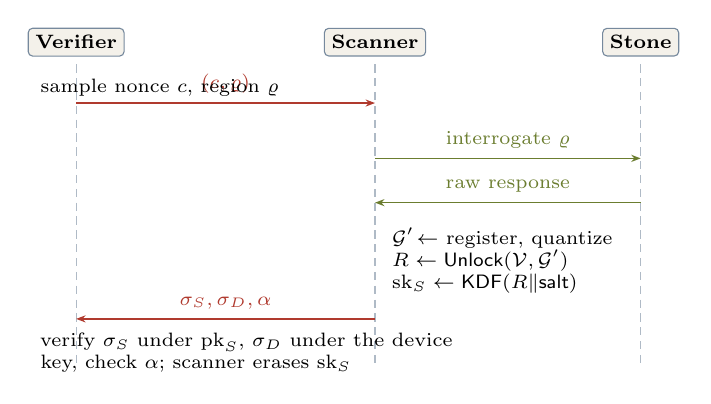
\begin{tikzpicture}[font=\scriptsize,x=1pt,y=1pt,
  hdr/.style={draw=Navy!60,fill=Pale,rounded corners=1.6pt,inner sep=2.6pt,font=\scriptsize\bfseries},
  msg/.style={-{Stealth[length=3.4pt]},semithick},
  note/.style={align=left,font=\scriptsize,inner sep=1pt}]
\def\xV{0}\def\xD{108}\def\xS{204}
\node[hdr] (V) at (\xV,0) {Verifier};
\node[hdr] (D) at (\xD,0) {Scanner};
\node[hdr] (S) at (\xS,0) {Stone};
\foreach \x in {\xV,\xD,\xS}{\draw[Navy!35,densely dashed] (\x,-8) -- (\x,-116);}
\draw[msg,Brick] (\xV,-22) -- node[above,font=\scriptsize]{$(c,\varrho)$} (\xD,-22);
\node[note,anchor=north west] at (\xV-14,-12) {sample nonce $c$, region $\varrho$};
\draw[msg,Olive] (\xD,-42) -- node[above,font=\scriptsize]{interrogate $\varrho$} (\xS,-42);
\draw[msg,Olive] (\xS,-58) -- node[above,font=\scriptsize]{raw response} (\xD,-58);
\node[note,anchor=north west,text width=104pt] at (\xD+5,-66)
  {$\mathcal{G}'\!\leftarrow$ register, quantize\\
   $R \leftarrow \textsf{Unlock}(\mathcal{V},\mathcal{G}')$\\
   $\mathrm{sk}_S \leftarrow \KDF(R\|\mathsf{salt})$};
\draw[msg,Brick] (\xD,-100) -- node[above,font=\scriptsize]{$\sigma_S,\sigma_D,\alpha$} (\xV,-100);
\node[note,anchor=north west,text width=150pt] at (\xV-14,-104)
  {verify $\sigma_S$ under $\mathrm{pk}_S$, $\sigma_D$ under the device key,
   check $\alpha$; scanner erases $\mathrm{sk}_S$};
\end{tikzpicture}
\caption{Verification. The verifier chooses both a nonce and an interrogation
region, so a stored measurement cannot answer, and the secret key exists only
transiently inside the attested device.}
\label{fig:proto}
\end{figure}

\subsection{Enrolment}

A certifying laboratory acquires $R$ scans across all three modalities,
constructs the Stage-A code and the Stage-B vault, derives $\mathrm{sk}_S$,
and publishes
\[
\mathsf{rec}_S = \big(\mathrm{pk}_S,\ H(\mathcal{V}),\ \mathsf{cls},\
H(\text{report}),\ \tau,\ \sigma_{\mathrm{lab}},\ \sigma_S \big),
\]
where $\mathcal{V}$ is the vault (stored off-chain, content-addressed),
$\mathsf{cls}$ is the $M_2$ material-class attestation, and $\tau$ is a
monotonic counter. The record is co-signed by the laboratory and by the stone.
Enrolment is the trust anchor and the point of maximum exposure to $A_8$, which
is why \Cref{sec:security} requires $k$-of-$n$ independent laboratories for
high-value stones.

\subsection{Challenged interrogation}

Freshness ($G_2$) and resistance to a compromised sensor ($A_5$) come from
making the measurement itself unpredictable. The verifier samples a region
$\varrho$: a sub-volume for $M_3$ confocal interrogation, together with an
excitation wavelength and, where applicable, a polarization setting. The
response is a hash over the measurement restricted to $\varrho$, signed under
both $\mathrm{sk}_S$ and the device attestation key. Because the challenge space
is large and the response depends on defect structure the protocol never
publishes, a replayed measurement from a different stone fails, and a
compromised scanner must synthesize a response for a region it has not seen.

The honest limit: an adversary with unrestricted physical access to the genuine
stone can characterize it exhaustively and then answer any challenge from a
compromised device. Challenged interrogation defends against remote and
partial-knowledge adversaries, not against $\mathcal{A}_{\mathrm{ins}}$ holding
the stone. We regard that residual as irreducible.

\subsection{Transfer, cloning, and re-cutting}

\paragraph{Transfer ($G_3$).} A custody transfer is a transaction signed by the
sender, the receiver, and the stone, incrementing $\tau$. Absent the physical
stone, no valid transfer exists.

\paragraph{Clone detection ($G_5$).} Cryptography cannot prevent physical
cloning; it can make cloning visible. Each verification appends a signed
$(\tau, \text{time}, \text{location}, \text{device})$ tuple. Two stones sharing
$\mathrm{pk}_S$ necessarily produce either a counter fork or a
spatiotemporally impossible pair of verifications. This is physical
double-spend detection, with the same guarantee structure: detection and
attribution after the fact rather than prevention.

\paragraph{Re-cutting ($G_6$).} \Cref{sec:eval} shows re-polishing drops vault
unlock probability from $0.97$ to $0.09$, so treating re-cut stones as
transparently re-verifiable is untenable. We instead require an explicit
transition: while the stone still satisfies the old key, it signs a transition
message committing to the new enrolment, witnessed by a laboratory. A re-cut
performed without this ceremony produces a stone with no valid record, which is
the correct outcome, since an unrecorded re-cut is indistinguishable from $A_7$.

\section{Security Analysis}
\label{sec:security}

\begin{description}[leftmargin=1.4em,style=nextline]
\item[$A_1$ Record forgery.] Requires a laboratory signature. Reduces to
laboratory key compromise; mitigated by $k$-of-$n$ certification and by public
transparency logs over enrolments.

\item[$A_2$ Substitution.] The substitute must unlock the vault. \Cref{sec:eval}
measures impostor unlock at $9.5\times10^{-5}$ for the chosen parameters, and
the $M_2$ gate independently rejects grown material at $99.8\%$ accuracy. The
2024 incident~\cite{igi2024} fails at both layers.

\item[$A_3$ Cloning.] Physical cloning of $M_1$ requires placing $\geq 20$
inclusions at specified positions inside a grown crystal; of $M_3$, atomic-scale
placement of $\sim 10^4$ colour centres. Neither is prevented by the protocol;
both are detected by $G_5$.

\item[$A_4$ Replay.] Defeated by nonce and region binding, provided the
challenge space is large relative to the adversary's stored measurements.

\item[$A_5$ Oracle compromise.] Constrained but not eliminated. Device
attestation plus unpredictable regions forces the adversary to synthesize
physically consistent responses. We consider this the weakest link and treat
$k$-of-$n$ multi-device verification as mandatory above a value threshold.

\item[$A_6$ Template inversion.] The gravest finding of \Cref{sec:eval}. Vault
security \Cref{eq:vaultsec} assumes the adversary cannot distinguish chaff from
genuine points. An adversary who independently learns a large fraction of the
inclusion map bypasses the vault entirely: at $90\%$ knowledge, unlock
probability is $0.49$. Clarity plots published on grading reports are precisely
such a partial map. Any deployment must therefore either withhold plot detail
below the lattice pitch, or draw the vault's genuine points from $M_3$ rather
than $M_1$. We regard this as a hard constraint on how the protocol may be
deployed alongside existing disclosure practice.

\item[$A_7$ Re-cut laundering.] Addressed by the transition ceremony; an
unwitnessed re-cut invalidates the record.

\item[$A_8$ Enrolment poisoning.] Mitigated by multi-laboratory enrolment and by
requiring that enrolment scans be individually attested.
\end{description}

\section{Evaluation}
\label{sec:eval}

\subsection{Methodology and its status}

We simulate $1{,}000$ stones: $500$ for fitting projections and quantization
thresholds, $500$ held out. Each stone has $K \sim \mathrm{Poisson}(18)$
inclusions, $60\%$ scattered through an anisotropic ellipsoid and $40\%$
concentrated on one or two growth planes, which imposes the spatial correlation
that suppresses true entropy relative to \Cref{eq:budget}. Each acquisition
applies a random rigid pose, per-axis localization noise
$\sigma = 8\,\mu$m, size-dependent detection failure (base rate $6\%$),
$\mathrm{Poisson}(0.6)$ spurious detections, and multiplicative size noise.
Enrolment uses $R=7$ scans and probing uses $5$. Re-polishing removes inclusions
within the outer $12\%$ of the radius and leaves the survivors rigid with
respect to one another, since polishing removes surface material rather than
deforming the lattice. Grown stones carry an $[\mathrm{SiV}]^-$ and $596/597$~nm
signature in the PL block.

\begin{quote}\small\itshape
These are simulation results on synthetic data. They are predictions about what
a physical study would find, conditional on a generative model that we chose.
They are not measurements of diamonds, and no claim here should be cited as
such.
\end{quote}

\subsection{Stage A: screening}

\Cref{fig:hamming} shows the Hamming geometry. Impostor distance concentrates at
$0.498 \pm 0.044$, as a well-balanced code should. Genuine re-scan distance is
$0.172$ at $n=64$, rising to $0.216$ as lower-reliability bits are admitted.

\begin{figure}[t]
\centering
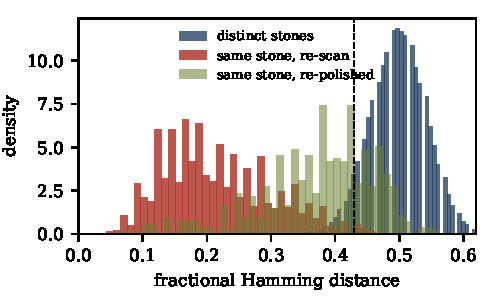
\includegraphics[width=\columnwidth]{fig_hamming.pdf}
\caption{Stage-A Hamming distance distributions ($n{=}135$). Genuine and
impostor populations separate cleanly, but re-polished stones sit between them,
foreshadowing the lifecycle problem addressed in \Cref{sec:protocol}.}
\label{fig:hamming}
\end{figure}

\begin{figure}[t]
\centering
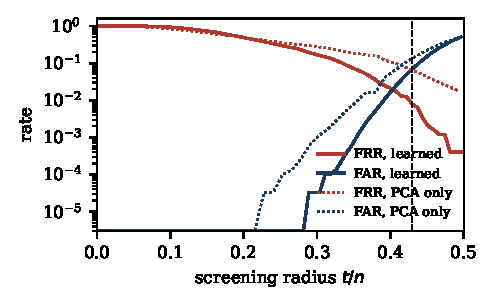
\includegraphics[width=\columnwidth]{fig_det.pdf}
\caption{Screening error rates. Learned within-class whitening improves the
equal error rate by $4.7\times$ over unsupervised whitening on the identical
descriptor.}
\label{fig:det}
\end{figure}

The supervised step matters. Within-class whitening lowers the equal error rate
from $8.9\times10^{-2}$ to $1.9\times10^{-2}$ on an identical raw descriptor
(\Cref{fig:det}), which isolates the gain to the projection rather than to
feature engineering. At a screening radius $t/n = 0.43$ with false rejection
$10^{-2}$, false acceptance is $6.9\times10^{-2}$, adequate for shortlisting a
registry and inadequate for anything else.

\paragraph{Finding 1: the alignment-free descriptor cannot bind.} Applying
\Cref{prop:feas} to the measured operating points, the best extractable key
length over all $n$ is $-124$ bits: the correlation-corrected entropy
($54.6$ bits at $n=64$, $106.4$ at $n=135$) never exceeds the sum of
error-correction leakage and extractor loss. \Cref{fig:feasible} places the
operating point far below every feasible contour. This is a structural result
rather than a tuning failure. Global invariants of a sparse point set discard
the very information that distinguishes stones, and no amount of downstream
cryptography recovers it.

\begin{figure}[t]
\centering
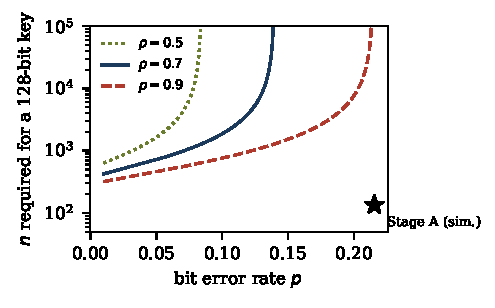
\includegraphics[width=\columnwidth]{fig_feasible.pdf}
\caption{Feasible region from \Cref{prop:feas} at $\ell{=}128$. The measured
Stage-A operating point (star) lies below every contour, so no code length makes
a single-stage fuzzy extractor over these invariants viable.}
\label{fig:feasible}
\end{figure}

\paragraph{Finding 2: the material-class gate must be spectroscopic.} All $200$
simulated CVD substitutes pass the geometric screen, with nearest-template
distance $0.365 \pm 0.018$ that is indistinguishable from any other impostor.
This is correct behaviour rather than a defect: a grown stone's inclusion
constellation is a different constellation, carrying no signature of how it was
made. The PL sub-block alone separates the classes at $99.8\%$ accuracy. Systems
that infer growth origin from geometry or from proportions are inferring it from
a variable that does not carry the information.

\subsection{Stage B: key extraction}

Registration succeeds with median residual $22.8\,\mu$m across $195$ evaluated
stones, yielding persistent templates of $|\mathcal{G}| = 14.1 \pm 3.9$ points
and a $91\,\mu$m lattice with $1.64\times10^5$ cells.

\begin{figure}[t]
\centering
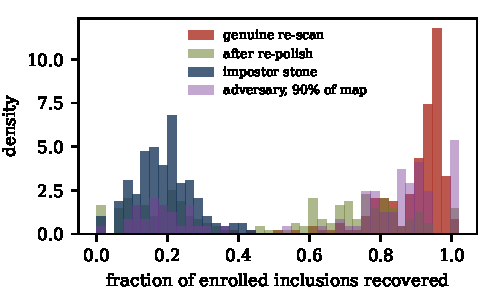
\includegraphics[width=\columnwidth]{fig_recovery.pdf}
\caption{Fraction of enrolled inclusions recovered. Genuine re-scans recover
$0.892$; impostors recover $0.187$, driven by lattice collisions rather than by
true correspondence; re-polished stones recover $0.479$; an adversary holding
$90\%$ of the map recovers $0.663$.}
\label{fig:recovery}
\end{figure}

\begin{figure}[t]
\centering
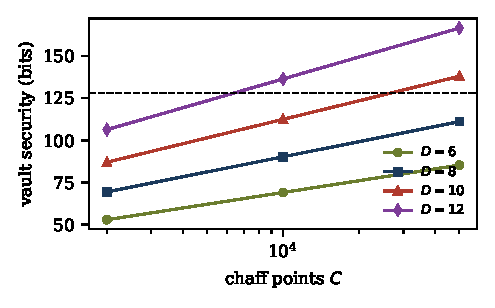
\includegraphics[width=\columnwidth]{fig_vault.pdf}
\caption{Vault security \Cref{eq:vaultsec} against chaff count. Higher $D$ and
higher $C$ both raise security and both lower the unlock probability through
\Cref{eq:decode}, so the usable region is bounded above by
\Cref{fig:recovery}.}
\label{fig:vault}
\end{figure}

\Cref{tab:vault} gives the joint operating characteristic. The best point
satisfying $\Pr[\text{unlock}] \geq 0.95$ is $C = 10^4$, $D = 8$, delivering
$90.2$-bit security with $0.970$ unlock and false unlock $9.5\times10^{-5}$.
Reaching $128$ bits at this $|\mathcal{G}|$ costs unlock probability: $C=10^4$,
$D=12$ gives $136.4$ bits at $0.288$ unlock, which is unusable.

\begin{table}[t]
\centering
\small
\setlength{\tabcolsep}{4.5pt}
\renewcommand{\arraystretch}{1.12}
\begin{tabular}{rrrrr}
\toprule
$C$ & $D$ & sec.\ (bits) & $\Pr[\text{unlock}]$ & $\Pr[\text{false}]$ \\
\midrule
$2{,}000$  & $8$  & $69.3$  & $0.995$ & $1.9\times10^{-4}$ \\
$10{,}000$ & $8$  & $90.2$  & $0.970$ & $9.5\times10^{-5}$ \\
$10{,}000$ & $10$ & $112.4$ & $0.779$ & $8.2\times10^{-7}$ \\
$10{,}000$ & $12$ & $136.4$ & $0.288$ & $1.5\times10^{-9}$ \\
$50{,}000$ & $10$ & $138.0$ & $0.106$ & $1.2\times10^{-8}$ \\
\bottomrule
\end{tabular}
\caption{Vault operating points at $|\mathcal{G}|=14$. Security and usability
are in direct conflict at this template size.}
\label{tab:vault}
\end{table}

\paragraph{Finding 3: security is an instrument specification.}
\Cref{fig:sens} sweeps $|\mathcal{G}|$ holding the recovery rate fixed. The
achievable security at $95\%$ unlock rises from $66.8$ bits at
$|\mathcal{G}|=10$ to $116.5$ at $18$ and $141.7$ at $22$, crossing $128$ bits
at $|\mathcal{G}| \approx 20$. The binding question is therefore not which
cryptographic construction to use but how many inclusions a mapper can resolve
\emph{reproducibly}, which is a specification a laboratory can procure against.
We note that commercial systems already claim micron-level detection on
rough~\cite{sarine_galaxy}, so the constraint plausibly lies in reproducibility
across instruments and settings rather than in raw sensitivity.

\begin{figure}[t]
\centering
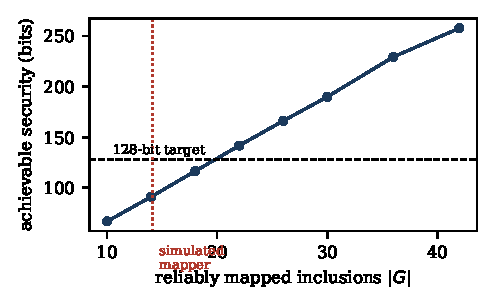
\includegraphics[width=\columnwidth]{fig_sens.pdf}
\caption{Achievable security against template size at fixed recovery rate,
maximized over $(C,D)$ subject to $\Pr[\text{unlock}] \geq 0.95$. Twenty
reliably mapped inclusions is the $128$-bit threshold.}
\label{fig:sens}
\end{figure}

\subsection{Adversarial stress tests}

\Cref{tab:attack} reports the partial-knowledge attack, in which an adversary
learns a fraction of the true inclusion map and fabricates the remainder. Unlock
probability is negligible below $50\%$ knowledge, rises steeply through $75\%$,
and reaches $0.487$ at $90\%$. The response is not steep enough to be
comfortable: the vault degrades gracefully from the adversary's point of view,
which is the wrong direction. This is the quantitative basis for the disclosure
constraint in \Cref{sec:security} and, in our view, the most important practical
result in the paper.

\begin{table}[t]
\centering
\small
\setlength{\tabcolsep}{6pt}
\renewcommand{\arraystretch}{1.12}
\begin{tabular}{rrr}
\toprule
Map known & Recovery & $\Pr[\text{unlock}]$ \\
\midrule
$25\%$ & $0.235 \pm 0.163$ & $5.9\times10^{-4}$ \\
$50\%$ & $0.266 \pm 0.191$ & $1.6\times10^{-3}$ \\
$75\%$ & $0.463 \pm 0.307$ & $7.7\times10^{-2}$ \\
$90\%$ & $0.663 \pm 0.325$ & $4.9\times10^{-1}$ \\
\bottomrule
\end{tabular}
\caption{Partial-knowledge attack at $C=10^4$, $D=8$.}
\label{tab:attack}
\end{table}

\subsection{Summary}

Stage A screens and classifies but cannot bind. Stage B binds at $90$ bits with
current template sizes and at $128$ bits given $\geq 20$ reliably mapped
inclusions. Neither stage survives re-polishing, which the protocol handles by
ceremony rather than by robustness. And the confidentiality goal $G_4$ is load
bearing in a way that the initial design underestimated.

\section{Deployment Considerations}
\label{sec:deploy}

\paragraph{Throughput and cost.} $M_1$ mapping is already in the manufacturing
path, so its marginal cost is near zero for stones that pass through planning.
$M_2$ adds a PL measurement at liquid-nitrogen temperature, routine in
laboratories and impractical in retail. $M_3$ requires confocal microscopy and
is a certification-time and dispute-time instrument. This tiering keeps the
common path cheap and reserves cost for the moments that carry value.

\paragraph{Interoperability with Tracr.} ADAMAS is complementary rather than
competing. Tracr establishes origin at source and follows the stone through
manufacture; ADAMAS supplies the missing cryptographic binding at each
checkpoint. Concretely, $\mathsf{rec}_S$ can be referenced from a Tracr asset
record, and Tracr's existing scanning integrations~\cite{debeers_tracr_case} are
where the attested-device requirement would be introduced.

\paragraph{Privacy and trade secrecy.} Dealers have legitimate reasons to hide
inventory and margins. Verification therefore proves a predicate, that this
stone corresponds to a record certified by an accredited laboratory and
currently held by the asserting party, without revealing the record's contents,
using standard succinct proofs over the on-chain
state~\cite{groth2016,zerocash2014}. We deliberately keep the fuzzy-extraction
computation outside the proof system, since proving a decoder in zero knowledge
buys little here and costs a great deal.

\section{Limitations and Threats to Validity}
\label{sec:limits}

\paragraph{The generative model is the main risk.} Real inclusion
constellations are not our mixture of ellipsoid and growth planes. If real
spatial correlation is stronger, extractable entropy falls and $|\mathcal{G}|$
must rise further; if inclusion counts in commercial goods are systematically
lower than $18$, the $128$-bit threshold may be out of reach for many stones,
which would push the design onto $M_3$ sooner. Our detection-failure and
spurious-detection rates are plausible but unmeasured.

\paragraph{We do not simulate $M_3$.} The claim that NV sub-volumes supply
$>10^4$ bits rests on defect-density arithmetic rather than on a simulated
readout pipeline with realistic confocal noise, drift, and charge-state
instability. The root of trust is therefore the least validated layer.

\paragraph{Fuzzy vault weaknesses.} Correlation attacks recover genuine points
from multiple enrolments of the same secret~\cite{scheirer2007}. Our protocol
re-enrolls after re-cutting, which is exactly the situation such attacks
exploit. Chaff must be regenerated under a fresh secret, and the number of
lifetime enrolments must be bounded.

\paragraph{The linear encoder understates achievable performance.} We used PCA
followed by within-class whitening in place of a trained equivariant encoder to
keep the ablation clean. A properly trained encoder should reduce BER and raise
$\rho$, though \Cref{prop:feas} bounds how much that can help: the entropy of
the underlying point set is what it is.

\paragraph{No physical validation.} Nothing here has touched a diamond.

\section{Research Plan}
\label{sec:plan}

The results above convert cleanly into an experimental program with a
gemological partner.

\paragraph{Phase 1 (months 1--4): measurement campaign.} Acquire repeated
inclusion maps of $\geq 1{,}000$ graded stones spanning clarity grades VVS
through I, with $\geq 5$ independent acquisitions per stone across $\geq 2$
instruments to separate within-instrument from between-instrument variance. The
primary deliverable is the empirical distribution of registration residual and
of reproducibly mapped inclusion count, which \Cref{fig:sens} shows is the
quantity that determines everything else.

\paragraph{Phase 2 (months 3--8): matched-pair studies.} Two subsets carry
disproportionate value. First, before-and-after pairs across re-polishing, which
determine whether $G_6$ can be relaxed from ceremony to robustness. Second,
adversarially matched pairs, i.e.\ grown stones selected or produced to resemble
specific natural targets in geometry, which measure the true $\mathcal{A}_{\mathrm{fab}}$
false-accept rate rather than the random-impostor rate we report.

\paragraph{Phase 3 (months 6--12): learned encoder.} Replace the linear
projection with an $E(3)$-equivariant graph encoder over the inclusion set,
trained with an angular-margin identity loss, an explicit bit-decorrelation
penalty targeting the $\rho$ term of \Cref{prop:feas}, and a reliability
weighting derived from repeated acquisitions. Success criterion: BER below $5\%$
at $\rho \geq 0.7$, which \Cref{tab:feas} shows suffices at $n \approx 720$.

\paragraph{Phase 4 (months 9--15): NV feasibility.} Establish on a small sample
whether an NV sub-volume can be re-located and re-measured reproducibly enough
to support challenge-response, which is the single assumption the root of trust
rests on and the one we have not tested.

\paragraph{Phase 5 (months 12--18): end-to-end pilot.} Instrument a real custody
chain with attested scanners and measure operational false-reject rates, which
in biometric systems invariably exceed laboratory estimates.

\section{Conclusion}

Ledger-based provenance secures the record and leaves the correspondence between
record and object to a trusted operator. We have argued that this gap is the
substantive security problem in diamond provenance, that closing it fully is
impossible, and that the reachable goal is a reduction of forgery to atomic-scale
replication, instrument compromise, or possession of the genuine stone.

ADAMAS pursues that reduction by deriving a key from crystallographic defect
structure and making possession of the stone a precondition for every provenance
operation. Simulation on $1{,}000$ synthetic stones supports the architecture and
sharpens it in three ways we did not anticipate. Alignment-free invariants are
structurally incapable of cryptographic binding, so registration is not an
implementation detail but the core of the design. Growth origin is invisible to
geometry and must be gated spectroscopically. And the threshold for $128$-bit
security is roughly twenty reproducibly mapped inclusions, which makes the
security level a procurement specification rather than a protocol choice.

The finding we would most want tested first is the disclosure risk. If an
adversary holding ninety percent of an inclusion map unlocks the vault half the
time, then publishing clarity plots and deploying an inclusion-derived key are
mutually incompatible, and the field should learn that before building the
system rather than after.

\section*{Reproducibility}

The simulation harness that produced every figure and table is a single
self-contained Python script with a fixed seed, released alongside this
manuscript.

\begin{thebibliography}{99}
\small
\setlength{\itemsep}{1pt}

\bibitem{pappu2002} R.~Pappu, B.~Recht, J.~Taylor, and N.~Gershenfeld.
Physical one-way functions. \emph{Science}, 297(5589):2026--2030, 2002.

\bibitem{gassend2002} B.~Gassend, D.~Clarke, M.~van~Dijk, and S.~Devadas.
Silicon physical random functions. In \emph{ACM CCS}, 2002.

\bibitem{suh2007} G.~E. Suh and S.~Devadas. Physical unclonable functions for
device authentication and secret key generation. In \emph{DAC}, 2007.

\bibitem{dodis2008} Y.~Dodis, L.~Reyzin, and A.~Smith. Fuzzy extractors: How to
generate strong keys from biometrics and other noisy data. \emph{SIAM Journal on
Computing}, 38(1):97--139, 2008.

\bibitem{juels1999} A.~Juels and M.~Wattenberg. A fuzzy commitment scheme. In
\emph{ACM CCS}, 1999.

\bibitem{juels2006} A.~Juels and M.~Sudan. A fuzzy vault scheme.
\emph{Designs, Codes and Cryptography}, 38(2):237--257, 2006.

\bibitem{maes2009} R.~Maes, P.~Tuyls, and I.~Verbauwhede. A soft decision helper
data algorithm for SRAM PUFs. In \emph{IEEE ISIT}, 2009.

\bibitem{ruhrmair2010} U.~R\"uhrmair, F.~Sehnke, J.~S\"olter, G.~Dror,
S.~Devadas, and J.~Schmidhuber. Modeling attacks on physical unclonable
functions. In \emph{ACM CCS}, 2010.

\bibitem{scheirer2007} W.~J. Scheirer and T.~E. Boult. Cracking fuzzy vaults and
biometric encryption. In \emph{Biometrics Symposium}, 2007.

\bibitem{nist90b} M.~S. Turan et al. Recommendation for the entropy sources used
for random bit generation. NIST SP 800-90B, 2018.

\bibitem{nakamoto2008} S.~Nakamoto. Bitcoin: A peer-to-peer electronic cash
system. 2008.

\bibitem{buterin2014} V.~Buterin. Ethereum: A next-generation smart contract and
decentralized application platform. 2014.

\bibitem{towncrier2016} F.~Zhang, E.~Cecchetti, K.~Croman, A.~Juels, and E.~Shi.
Town Crier: An authenticated data feed for smart contracts. In \emph{ACM CCS},
2016.

\bibitem{zerocash2014} E.~Ben-Sasson, A.~Chiesa, C.~Garman, M.~Green, I.~Miers,
E.~Tromer, and M.~Virza. Zerocash: Decentralized anonymous payments from
Bitcoin. In \emph{IEEE S\&P}, 2014.

\bibitem{groth2016} J.~Groth. On the size of pairing-based non-interactive
arguments. In \emph{EUROCRYPT}, 2016.

\bibitem{doherty2013} M.~W. Doherty, N.~B. Manson, P.~Delaney, F.~Jelezko,
J.~Wrachtrup, and L.~C.~L. Hollenberg. The nitrogen-vacancy colour centre in
diamond. \emph{Physics Reports}, 528(1):1--45, 2013.

\bibitem{balasubramanian2008} G.~Balasubramanian et al. Nanoscale imaging
magnetometry with diamond spins under ambient conditions. \emph{Nature},
455:648--651, 2008.

\bibitem{maurer2012} P.~C. Maurer et al. Room-temperature quantum bit memory
exceeding one second. \emph{Science}, 336(6086):1283--1286, 2012.

\bibitem{zaitsev2001} A.~M. Zaitsev. \emph{Optical Properties of Diamond: A Data
Handbook}. Springer, 2001.

\bibitem{breeding2009} C.~M. Breeding and J.~E. Shigley. The ``type''
classification system of diamonds and its importance in gemology. \emph{Gems \&
Gemology}, 45(2):96--111, 2009.

\bibitem{breeding2008} C.~M. Breeding and W.~Wang. Occurrence of the Si-V defect
center in natural colorless gem diamonds. \emph{Diamond and Related Materials},
17(7--10):1335--1344, 2008.

\bibitem{martineau2004} P.~M. Martineau et al. Identification of synthetic
diamond grown using chemical vapor deposition (CVD). \emph{Gems \& Gemology},
40(1):2--25, 2004.

\bibitem{gia_pl2016} S.~Eaton-Maga\~na and C.~M. Breeding. An introduction to
photoluminescence spectroscopy for diamond and its applications in gemology.
\emph{Gems \& Gemology}, 52(1), 2016.

\bibitem{gia_pl2024} S.~Eaton-Maga\~na et al. Shining a light on gemstone
properties: An exploration of photoluminescence spectroscopy. \emph{Gems \&
Gemology}, 60(4), 2024.

\bibitem{gia_cvd2016} S.~Eaton-Maga\~na and J.~E. Shigley. Observations on
CVD-grown synthetic diamonds: A review. \emph{Gems \& Gemology}, 52(3), 2016.

\bibitem{gia_cvd2023} GIA Laboratory. CVD-grown diamond with few diagnostic
features. \emph{Gems \& Gemology} Lab Notes, Fall 2023.

\bibitem{gia_si2013} GIA Laboratory. Silicon in natural type IIa and type IaB
diamond. \emph{Gems \& Gemology} Lab Notes, Winter 2013.

\bibitem{igi2024} International Gemological Institute. IGI uncovers fraudulent
6~ct laboratory-grown diamond bearing a natural diamond inscription. 2024.
\url{https://www.igi.org/igi-uncovers-fraudulent-6ct-lab-grown-diamond-with-natural-inscription/}

\bibitem{gia2026} Gemological Institute of America. GIA acquires 30\%
shareholding in diamond provenance blockchain platform Tracr. Press release,
May~29, 2026. \url{https://www.gia.edu/gia-news-press/gia-and-tracr}

\bibitem{debeers2026} De Beers Group. GIA acquires 30 percent shareholding in
diamond provenance blockchain platform Tracr. May~29, 2026.

\bibitem{debeers_tracr_case} De Beers Group. Tracr: Diamond traceability
platform. Case study, 2024.

\bibitem{tnw2026} The Next Web. De Beers weaponises blockchain to fight
lab-grown diamonds. June~2026.

\bibitem{sarine_galaxy} Sarine Technologies. Galaxy Ultra inclusion mapping
system. Product documentation.

\bibitem{sarine_tech} Sarine Technologies. Technology overview: Galaxy,
DiaExpert, DiaMension.

\bibitem{sarine_journey} Sarine Technologies. Sarine Diamond Journey:
traceability and polished validation.

\bibitem{nanodiamond2024} Authors of ``High-dimensional anticounterfeiting
nanodiamonds authenticated with deep metric learning.'' \emph{Nature
Communications}, 15, 2024.

\bibitem{siv_puf2023} Authors of ``Manufacturing unclonable anti-counterfeiting
labels using robust diamond microparticles on heterogeneous substrates.'' 2023.

\bibitem{satorras2021} V.~G. Satorras, E.~Hoogeboom, and M.~Welling. E(n)
equivariant graph neural networks. In \emph{ICML}, 2021.

\bibitem{zaheer2017} M.~Zaheer, S.~Kottur, S.~Ravanbakhsh, B.~P\'oczos,
R.~Salakhutdinov, and A.~Smola. Deep sets. In \emph{NeurIPS}, 2017.

\bibitem{qi2017} C.~R. Qi, H.~Su, K.~Mo, and L.~J. Guibas. PointNet: Deep
learning on point sets for 3D classification and segmentation. In \emph{CVPR},
2017.

\bibitem{deng2019} J.~Deng, J.~Guo, N.~Xue, and S.~Zafeiriou. ArcFace: Additive
angular margin loss for deep face recognition. In \emph{CVPR}, 2019.

\end{thebibliography}

\onecolumn
\appendix

\section{Protocol Pseudocode}

\begin{algorithm}[H]
\caption{$\textsf{Enroll}(S)$ --- executed by a certifying laboratory}
\begin{algorithmic}[1]
\State acquire $M_1$ scans $\{s_1,\dots,s_R\}$, $M_2$ spectrum $\pi$, $M_3$ reference map $\nu$
\State $\mathsf{cls} \gets \textsf{ClassGate}(\pi)$ \Comment{natural / CVD / HPHT / treated}
\If{$\mathsf{cls} \neq \textsf{natural}$ and origin claim is natural} \textbf{abort} \EndIf
\State $\mathcal{G} \gets \textsf{FuseTemplate}(s_1,\dots,s_R)$ \Comment{register, quantize, keep persistent points}
\If{$|\mathcal{G}| < G_{\min}$} \textbf{abort} \Comment{$G_{\min}=20$ per \Cref{fig:sens}} \EndIf
\State sample $\Phi \xleftarrow{\$} \mathrm{GF}(q)[x]$ of degree $D$; $R_{\mathrm{key}} \gets \textsf{Encode}(\Phi)$
\State $\mathcal{V} \gets \{(g,\Phi(g)) : g \in \mathcal{G}\} \cup \textsf{Chaff}(C)$
\State $\mathrm{sk}_S \gets \KDF(R_{\mathrm{key}} \Vert \mathsf{salt})$; \; $\mathrm{pk}_S \gets \textsf{Pub}(\mathrm{sk}_S)$
\State $\mathsf{rec}_S \gets (\mathrm{pk}_S, H(\mathcal{V}), \mathsf{cls}, H(\nu), H(\text{report}), \tau{=}0)$
\State publish $\mathsf{rec}_S$ signed by the laboratory and by $\mathrm{sk}_S$; \textbf{erase} $\mathrm{sk}_S, R_{\mathrm{key}}, \Phi$
\end{algorithmic}
\end{algorithm}

\begin{algorithm}[H]
\caption{$\textsf{Verify}(S, \mathsf{rec}_S)$ --- verifier $V$ and attested device $\mathcal{D}$}
\begin{algorithmic}[1]
\State $V$: sample nonce $c \xleftarrow{\$} \bits^{128}$ and interrogation region $\varrho \xleftarrow{\$} \mathcal{R}$; send $(c,\varrho)$
\State $\mathcal{D}$: acquire $M_1$ scan $s'$ and $M_3$ response $\nu'$ restricted to $\varrho$
\State $\mathcal{D}$: $\mathcal{G}' \gets \textsf{Register}(s', \text{helper})$; \; $\Phi' \gets \textsf{RSDecode}(\mathcal{V}, \mathcal{G}')$
\If{decoding fails} \textbf{return} $\bot$ \EndIf
\State $\mathcal{D}$: $\mathrm{sk}_S \gets \KDF(\textsf{Encode}(\Phi') \Vert \mathsf{salt})$
\State $\mathcal{D}$: $\sigma_S \gets \Sign_{\mathrm{sk}_S}(c \Vert \varrho \Vert H(\nu') \Vert \tau)$, \;
       $\sigma_D \gets \Sign_{\mathrm{sk}_\mathcal{D}}(\sigma_S \Vert \alpha)$
\State $\mathcal{D}$: \textbf{erase} $\mathrm{sk}_S, \Phi'$; send $(\sigma_S, \sigma_D, \alpha, H(\nu'))$
\State $V$: \textbf{return} $\Vf_{\mathrm{pk}_S}(\sigma_S) \wedge \Vf_{\mathcal{D}}(\sigma_D)
       \wedge \textsf{CheckAttest}(\alpha) \wedge \textsf{ConsistentNV}(H(\nu'), \varrho)$
\end{algorithmic}
\end{algorithm}

\begin{algorithm}[H]
\caption{$\textsf{Transfer}(S, P_{\mathrm{from}}, P_{\mathrm{to}})$ and $\textsf{Recut}(S)$}
\begin{algorithmic}[1]
\State \textbf{Transfer:} run $\textsf{Verify}$; on success submit
       $(\mathsf{rec}_S, \tau{+}1, P_{\mathrm{to}})$ signed by $\mathrm{sk}_S$,
       $P_{\mathrm{from}}$, and $P_{\mathrm{to}}$
\State ledger rejects any transfer whose $\tau$ is not the successor of the recorded value
\Statex
\State \textbf{Recut:} \emph{before} polishing, run $\textsf{Verify}$ and emit
       $\sigma_{\mathrm{trans}} \gets \Sign_{\mathrm{sk}_S}(\textsf{``intent-to-recut''} \Vert \mathsf{plan})$
\State after polishing, run $\textsf{Enroll}$ to obtain $\mathrm{pk}_{S'}$
\State publish $(\mathrm{pk}_S \to \mathrm{pk}_{S'})$ carrying $\sigma_{\mathrm{trans}}$ and a laboratory witness signature
\State mark $\mathrm{pk}_S$ retired; any later verification under $\mathrm{pk}_S$ is a clone signal
\end{algorithmic}
\end{algorithm}

\section{Simulation Parameters}

\begin{table}[H]
\centering
\small
\setlength{\tabcolsep}{8pt}
\renewcommand{\arraystretch}{1.15}
\begin{tabular}{llll}
\toprule
Parameter & Symbol & Value & Role \\
\midrule
Stone half-dimension        & $R$              & $2500\,\mu$m & sets the position space \\
Inclusion count             & $K$              & $\mathrm{Poisson}(18)$, clipped $[6,45]$ & entropy source size \\
Growth-plane fraction       & ---              & $0.40$ & imposes spatial correlation \\
Ellipsoid anisotropy        & ---              & $(1.00, 0.84, 0.63)$ & stabilizes the canonical frame \\
Localization noise          & $\sigma$         & $8\,\mu$m per axis & mapper precision \\
Detection failure (base)    & $p_{\mathrm{miss}}$ & $0.06$, size-scaled & deletions \\
Spurious detections         & ---              & $\mathrm{Poisson}(0.6)$ & insertions \\
Size measurement noise      & ---              & $\mathrm{LogNormal}(0, 0.12)$ & weight perturbation \\
Enrolment / probe scans     & $R_e / R_p$      & $7 / 5$ & template quality \\
Re-polish depth             & ---              & outer $12\%$ of radius removed & lifecycle test \\
Population                  & ---              & $500$ train $/$ $500$ test & fit / evaluation split \\
Raw descriptor dimension    & $d$              & $326$ & Stage-A input \\
PCA subspace                & $d'$             & $275$ & rank reduction \\
Bit allocation thresholds   & ---              & $\mathrm{SNR} > \{1,2,4\}$ & $k_j \in \{0,1,2,3\}$ \\
Correspondence tolerance    & ---              & $120\,\mu$m & Stage-B matching \\
Lattice pitch               & $\lambda$        & $4\bar{r} \approx 91\,\mu$m & quantization \\
Rotation hypotheses         & ---              & $24$ & proper signed permutations \\
Random seed                 & ---              & $20260721$ & reproducibility \\
\bottomrule
\end{tabular}
\end{table}

\end{document}
